%%%%%%%%%%%%%%%%%%%%%%
%%%%%%%%%%%%%%%%%%%%%%
%%Options for presentations (in-class) and handouts (e.g. print). 
\documentclass[pdf
%,handout
]{beamer}
\usepackage{pgfpages}
%\pgfpagesuselayout{2 on 1}[letterpaper,border shrink=5mm]

\graphicspath{{../}}
%%%%%%%%%%%%%%%%%%%%%%
%% Change this for different slides so it appears in bar
\usepackage{authoraftertitle}
\date{5.1, 5.2, and 5.4 (partial)\\ Linear Transformations and Matrices}

%%%%%%%%%%%%%%%%%%%%%%
%% Upload common style file
\usepackage{../LyryxLinearAlgebraSlidesStyle}

\usepackage{multirow}
\begin{document}
	
	%%%%%%%%%%%%%%%%%%%%%%%
	%% Title Page and Copyright Common to All Slides
	
	%Title Page
	\input ../frontmatter/titlepage.tex
	
	%LOTS Page
	%\input frontmatter/lyryxopentexts.tex
	
	%Copyright Page
	\input ../frontmatter/copyright.tex
	
	%%%%%%%%%%%%%%%%%%%%%%%%%


%\section{Introduction}
%%-------------- start slide -------------------------------%
%\frame{
%\begin{block}{Notation and Terminology}
%\pause 
%\begin{itemize}
%\item We have already used \alert{$\RR$} to denote the set 
%of \alert{real numbers}.
%\pause 
%\item We use \alert{$\RR^2$} to the denote the set of
%all \alert{column vectors of length two},
%\pause
% and we use
%\alert{$\RR^3$} to the denote the set of
%all \alert{column vectors of length three}
%\pause
%\textcolor{blue}{(the length of a vector is the number
%of entries it contains).}
%\pause
%\item In general, we write \alert{$\RR^n$} for the
%set of all \alert{column vectors of length $n$}.
%\end{itemize}
%\end{block}
%\pause
%\begin{alertblock}{$\RR^2$ and $\RR^3$}
%Vectors in $\RR^2$ and $\RR^3$ have convenient geometric
%interpretations as {\bf position vectors} of points in
%the 2-dimensional (Cartesian) plane and in 3-dimensional
%space, respectively.
%\end{alertblock}
%}
%%-------------- end slide -------------------------------%
%
%%-------------- start slide -------------------------------%
%\frame{%\frametitle{Geometric Vectors in $\RR^2$ and $\RR^3$}
%\begin{picture}(4,2.5)
%\put(0.3,0.7){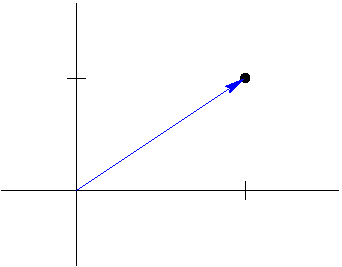
\includegraphics[scale=0.7]{figures/R2.pdf}}
%\put(0.2,2.2){{$\RR^2$}}
%\put(0.5,0.9){\scriptsize{$0$}}
%\put(1.7,0.95){\scriptsize{$x$}}
%\put(1.4,0.9){\scriptsize{$a$}}
%\put(0.55,1.9){\scriptsize{$y$}}
%\put(0.5,1.55){\scriptsize{$b$}}
%\put(1.5,1.6){\scriptsize{\alert{$(a,b)$}}}
%\pause
%\put(0.5,0.3){\scriptsize\textcolor{blue}{The vector 
%$\left[\begin{array}{c} a \\ b\end{array}\right]$.}} 
%\pause
%\put(2.4,2.4){{$\RR^3$}}
%\put(2.5,0.3){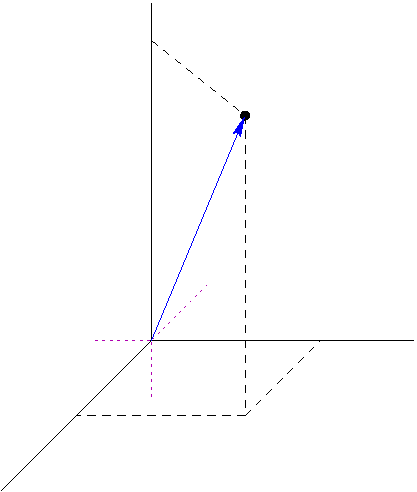
\includegraphics[scale=0.7]{figures/R3.pdf}}
%\put(3.05,1.1){\scriptsize{$0$}}
%\put(2.45,0.4){\scriptsize{$x$}}
%\put(4.3,0.9){\scriptsize{$y$}}
%\put(3.18,2.65){\scriptsize{$z$}}
%\put(3.75,2.05){\scriptsize{\alert{$(a,b,c)$}}}
%\put(2.7,0.65){\scriptsize{$a$}}
%\put(3.95,1.05){\scriptsize{$b$}}
%\put(3.05,2.45){\scriptsize{$c$}}
%\pause
%\put(3.0,0.1){\scriptsize\textcolor{blue}{The vector 
%$\left[\begin{array}{c} a \\ b \\c \end{array}\right]$.}} 
%\end{picture}
%}
%%-------------- end slide -------------------------------%

\section{Transformations}

%-------------------start slide-------------------%
\frame{\frametitle{Transformation by Matrix Multiplication}
\begin{example}
Consider the matrix $A = \left[
\begin{array}{rrr}
1 & 2 & 0 \\
2 & 1 & 0 
\end{array}
\right]$. By matrix multiplication, $A$ transforms vectors in $\mathbb{R}^3$ into vectors in $\mathbb{R}^2$. 

\pause

Consider the vector $\left[
\begin{array}{c}
x \\
y \\
z
\end{array}
\right]$. Transforming this vector by $A$ looks like:
\[
\left[
\begin{array}{rrr}
1 & 2 & 0 \\
2 & 1 & 0 
\end{array}
\right]
\left[
\begin{array}{c}
x \\
y \\
z
\end{array}
\right]
=
\left[
\begin{array}{c}
x + 2y \\
2x + y 
\end{array}
\right]
\]
\pause

For example:
\[
\left[
\begin{array}{rrr}
1 & 2 & 0 \\
2 & 1 & 0 
\end{array}
\right]
\left[
\begin{array}{c}
1 \\
2 \\
3
\end{array}
\right]
=
\left[
\begin{array}{c}
5 \\
4 
\end{array}
\right]
\]
\end{example}
}
%--------------------end slide---------------------%

%-------------- start slide -------------------------------%
\frame{\frametitle{Transformations}
\begin{definition}
A \alert{transformation} is a function
$T:\RR^n\rightarrow \RR^m$, sometimes written
\vspace*{-.1in}

\[ \RR^n\stackrel{T}{\rightarrow} \RR^m,\]
\vspace*{-.2in}

and is called a \alert{transformation from $\RR^n$
to $\RR^m$.}
\pause
If $m=n$, then we say \alert{$T$ is a transformation
of $\RR^n$.}
\end{definition}
\pause
\begin{alertblock}{What do we mean by a function?}
\pause
Informally, a function $T:\RR^n\to\RR^m$ is a rule that
assigns exactly one vector of $\RR^m$ to each vector of
$\RR^n$. \\
We use the notation $T(\vect{x})$ to mean the transformation $T$ applied to the vector $\vect{x}$. 
\end{alertblock}
\pause
\begin{definition}
If $T$ acts by matrix multiplication of a matrix $A$ (such as the previous example), we call $T$ a \alert{matrix transformation},
and write $T_A(\vect{x}) = A\vect{x}$. 
\end{definition}
}


%-------------- end slide -------------------------------%

%-------------- start slide -------------------------------%
\frame{\frametitle{Equality of Transformations}
\begin{definition}
Suppose $S:\RR^n\rightarrow\RR^m$
and $T:\RR^n\rightarrow\RR^m$
are transformations.
Then $S=T$ if and only if $S(\vect{x})=T(\vect{x})$ for every $\vect{x}\in\RR^n$.
\end{definition}
}
%-------------- end slide -------------------------------%


%-------------- start slide -------------------------------%
{\small
\frame{\frametitle{Specifying the Action of a Transformation}
\begin{example}
$T:\RR^3\rightarrow\RR^4$ defined by
\[
T\left[\begin{array}{c} a \\ b\\ c\end{array}\right]
=\left[ \begin{array}{c} 
a+b \\ b+c \\ a-c\\ c-b \end{array}\right]
\]
is a transformation
\pause
that \alert{transforms} the vector $\left[ \begin{array}{r}
1 \\ 4 \\ 7
\end{array}
\right]$ in $\RR^3$ 
into the vector
\[
T\left[\begin{array}{r} 1 \\ 4\\ 7\end{array}\right]
=\left[ \begin{array}{r}
1 + 4 \\ 4+7 \\ 1-7\\ 7-4 \end{array}\right]
=\left[ \begin{array}{r} 
5 \\ 11 \\ -6 \\ 3 \end{array}\right].
\]
\end{example}
}}
%-------------- end slide -------------------------------%

\section{Linear Transformations}

%-------------- start slide -------------------------------%
\frame{\frametitle{Linear Transformations}
\begin{definition}
\pause
A transformation $T:\RR^n\rightarrow \RR^m$ is a
\alert{linear transformation} if it satisfies the following
two properties for all $\vect{x},\vect{y}\in\RR^n$ and all (scalars) $a\in\RR$.
\pause
\begin{enumerate}
\item $T(\vect{x}+\vect{y})=T(\vect{x})+T(\vect{y})$ \hfill\alert{(preservation of addition)}
\pause
\item $T(a\vect{x})=aT(\vect{x})$
\hfill\alert{(preservation of scalar multiplication)}
\end{enumerate}
\end{definition}
}
%-------------- end slide -------------------------------%


%-------------- start slide -------------------------------%
\frame{
\begin{block}{Properties of Linear Transformations}
Let $T:\RR^n\to\RR^m$ be a linear transformation, and
let $\vect{x}\in\RR^n$.
\pause
Since $T$ preserves scalar multiplication,
\begin{enumerate}
\pause
\item $T(0\vect{x})=0T(\vect{x})$ implying $T(\vec{0})=\vec{0}$, 
so \alert{$T$ preserves the zero vector}.
\pause
\item $T((-1)\vect{x})=(-1)T(\vect{x})$, implying $T(-\vect{x})=-T(\vect{x})$,
so \alert{$T$ preserves the negative of a vector}.
\end{enumerate}
\pause
Suppose $\vect{x}_1, \vect{x}_2, \ldots, \vect{x}_k$ are vectors in $\RR^n$
and \[ \vect{y} = a_1\vect{x}_1 + a_2\vect{x}_2 +\cdots + a_k\vect{x}_k\] 
for some $a_1, a_2, \ldots, a_k\in\RR$.
\pause
Then 
\begin{enumerate}
\setcounter{enumi}{2}
\item
\[ \begin{array}{rcl}
T(\vect{y}) & = & T(a_1\vect{x}_1 + a_2\vect{x}_2 +\cdots + a_k\vect{x}_k) \\
& = & a_1T(\vect{x}_1) + a_2T(\vect{x}_2)+\cdots + a_kT(\vect{x}_k),
\end{array}\]
i.e.,\alert{$T$ preserves linear combinations.}
\end{enumerate}
\end{block}
}
%-------------- end slide -------------------------------%

%-------------- start slide -------------------------------%
{\small
\frame{
\begin{problem}\em
Let $T:\RR^3 \rightarrow \RR^4$ be a linear transformation
such that
\[ T\left[\begin{array}{r}
1 \\ 3 \\ 1
\end{array}\right] 
=
\left[\begin{array}{r}
4 \\ 4\\ 0 \\ -2
\end{array}\right]
\mbox{ and }
T\left[\begin{array}{r}
4 \\ 0 \\ 5 
\end{array}\right]
=
\left[\begin{array}{r}
4 \\ 5 \\ -1 \\ 5 
\end{array}\right].
\pause
\mbox{ Find }
T\left[\begin{array}{r}
-7 \\ 3 \\ -9
\end{array}\right].\]
\end{problem}
\pause
\begin{solution}\em
\pause
The only way it is possible to solve this problem is if
\[ \left[\begin{array}{r}
-7 \\ 3 \\ -9
\end{array}\right]
\mbox{ is a linear combination of }
\left[\begin{array}{r}
1 \\ 3 \\ 1 
\end{array}\right]
\mbox{ and }
\left[\begin{array}{r}
4 \\ 0 \\ 5 
\end{array}\right],\] 
\vspace*{-.1in}

\pause
i.e., if there exist $a,b\in\RR$ so that
\vspace*{-.1in}

 \[ \left[\begin{array}{r}
-7 \\ 3 \\ -9 
\end{array}\right]
=
a\left[\begin{array}{r}
1 \\3 \\ 1
\end{array}\right]
+
b\left[\begin{array}{r}
4 \\ 0 \\ 5
\end{array}\right].
\] 
\end{solution}
}}
%-------------- end slide -------------------------------%

%-------------- start slide -------------------------------%
{\small
\frame{
\begin{solution}[continued]\em
To find $a$ and $b$, solve the system of three
equations in two variables:
\[
\left[\begin{array}{rr|r}
1 & 4 & -7 \\
3 & 0 & 3 \\
1 & 5 & -9
\end{array}\right] 
\rightarrow \cdots \rightarrow
\left[\begin{array}{rr|r}
1 & 0 & 1 \\
0 & 1 & -2 \\
0 & 0 & 0 
\end{array}\right] 
\]
Thus $a=1$, $b=-2$, and
\[ \left[\begin{array}{r}
-7 \\ 3 \\ -9
\end{array}\right]
=
\left[\begin{array}{r}
1 \\ 3 \\ 1
\end{array}\right]
-
2\left[\begin{array}{r}
4 \\ 0 \\ 5 
\end{array}\right].
\] 
\end{solution}
}
%-------------- end slide -------------------------------%

%-------------- start slide -------------------------------%
{\small
\frame{
\begin{solution}[continued]\em
We now use that fact that linear transformations preserve
linear combinations, implying that
\begin{eqnarray*}
T \left[\begin{array}{r}
-7 \\ 3 \\ -9
\end{array}\right]
& = &
T\left(
\left[\begin{array}{r}
1 \\ 3 \\ 1
\end{array}\right]
-
2\left[\begin{array}{r}
4 \\ 0 \\ 5 
\end{array}\right]\right)\\
\pause
& = &
T \left[\begin{array}{r}
1 \\ 3 \\ 1 
\end{array}\right]
- 2T\left[\begin{array}{r}
4 \\ 0 \\ 5 
\end{array}\right] \\
\pause
& = &
\left[\begin{array}{r}
4 \\ 4 \\ 0 \\ -2
\end{array}\right]
- 2\left[\begin{array}{r}
4 \\ 5 \\ -1 \\ 5 
\end{array}\right] 
=
\left[\begin{array}{r}
-4 \\ -6 \\ 2 \\ -12 
\end{array}\right]
\end{eqnarray*}
\pause
Therefore, 
$T \left[\begin{array}{r}
-7 \\ 3 \\ -9
\end{array}\right]
= \left[\begin{array}{r}
-4 \\ -6 \\ 2 \\ -12
\end{array}\right]$.
\end{solution}
}}
%-------------- end slide -------------------------------%

%-------------- start slide -------------------------------%
{\small
\frame{
\begin{problem}\em
Let $T:\RR^4 \rightarrow \RR^3$ be a linear transformation
such that
\[ T\left[\begin{array}{r}
1\\1\\ 0 \\ -2
\end{array}\right] 
=
\left[\begin{array}{r}
2 \\ 3 \\ -1
\end{array}\right]
\mbox{ and }
T\left[\begin{array}{r}
0\\-1 \\ 1 \\ 1 
\end{array}\right]
=
\left[\begin{array}{r}
5 \\ 0 \\ 1
\end{array}\right].
\mbox{ Find }
T\left[\begin{array}{r}
2 \\ 5 \\ -3\\-7
\end{array}\right].\]
\end{problem}
\pause
\begin{block}{Final Answer}
\[ T\left[\begin{array}{r}
2 \\ 5 \\ -3\\-7 % = 2 u - 3 v 
\end{array}\right]
=\left[\begin{array}{r}
-11 \\ 6 \\ -5
\end{array}\right].\]
\end{block}
}}
%-------------- end slide -------------------------------%



%-------------- start slide -------------------------------%
\frame{\frametitle{Matrix Transformations}
\begin{theorem}\em
Every matrix transformation is a linear transformation.
\end{theorem}
\pause
\begin{proof}
Suppose $T:\RR^n\rightarrow\RR^m$ is a matrix transformation
induced by the $m\times n$ matrix $A$,
i.e., $T(\vect{x})=A\vect{x}$ for each $\vect{x}\in\RR^n$.
\pause
Let $\vect{x},\vect{y}\in\RR^n$ and let $a\in\RR$.
\pause
Then
\[ T(\vect{x}+\vect{y})=A(\vect{x}+\vect{y})=A\vect{x}+A\vect{y}=T(\vect{x})+T(\vect{y}),\]
proving that $T$ preserves addition.
\pause
Also,
\[ T(a\vect{x})=A(a\vect{x})=a(A\vect{x})=aT(\vect{x}),\]
proving that $T$ preserves scalar multiplication.
\pause
\bigskip

Since $T$ preserves addition and scalar multiplication
$T$ is a linear transformation.
\end{proof}
}
%-------------- end slide -------------------------------%



%-------------- start slide -------------------------------%
\frame{\frametitle{Some Special Matrix Transformations}
\begin{example}[The Zero Transformation]
If $A$ is the $m \times n$ matrix of zeros,
then the transformation $T:\RR^n\to\RR^m$ induced by $A$ 
is called the \alert{zero transformation} because
for every vector $\vect{x}$ in $\RR^n$
\[ T(\vect{x}) = A\vect{x} = 0\vect{x} = \vect{0}. \]
\pause
\textcolor{blue}{Note that the first zero is the matrix $A$, while
the second zero is the zero vector of $\RR^m$.}
 
The zero transformation is usually written as \alert{$T=0$}.
\end{example}
\pause
\begin{example}[The Identity Transformation]
The transformation of $\RR^n$ induced by $I_n$, the 
$n\times n$ identity matrix,
is called the \alert{identity transformation}
because for every vector $\vect{x}$ in $\RR^n$,
\[ T(\vect{x}) = I_n\vect{x}=\vect{x}.  \]
 
The identity transformation on $\RR^n$ is usually written
as \alert{$1_{\RR^n}$}.
\end{example}
}
%-------------- end slide -------------------------------%


%-------------- start slide -------------------------------%
{\small
\begin{example}[Revisited]
Recall $T:\RR^3\rightarrow\RR^4$ defined by
\[
T\left[\begin{array}{c} a \\ b\\ c\end{array}\right]
=\left[ \begin{array}{c} 
a+b \\ b+c \\ a-c\\ c-b \end{array}\right]
\]

\pause

\alert{Is $T$ a matrix transformation?}

\smallskip

\pause 

Consider $A= 
\left[ \begin{array}{rrr}
1 & 1 & 0 \\
0 & 1 & 1 \\
1 & 0 & -1 \\
0 & -1 & 1 \\
\end{array}
\right]$, then 

\[
A\left[\begin{array}{r} a \\ b\\ c \end{array}\right]
=
\left[ \begin{array}{rrr}
1 & 1 & 0 \\
0 & 1 & 1 \\
1 & 0 & -1 \\
0 & -1 & 1 \\
\end{array}
\right]
\left[\begin{array}{r} a \\ b\\ c \end{array}\right]
=
\left[ \begin{array}{c} 
a+b \\ b+c \\ a-c\\ c-b \end{array}\right]
=
T\left[\begin{array}{c} a \\ b\\ c\end{array}\right]
\]

\pause 

\alert{So in this case $T$ is a matrix transformation!}
\end{example}
}}
%-------------- end slide -------------------------------%



%-------------- start slide -------------------------------%
\frame{
\frametitle{\alert{Not all transformations are matrix  transformations!}}

\begin{example}
  
Consider $T:\RR^2 \rightarrow \RR^2$ defined by
\[ T(\vect{x}) = \vect{x} + 
\left[\begin{array}{r} 1 \\ -1 \end{array}\right]
\mbox{ for all } \vect{x}\in\RR^2.\]

\pause

\begin{center}
\alert{Why is $T$ not a matrix transformation?}
\end{center}

\end{example}

}
%-------------- end slide -------------------------------%



%-------------- start slide -------------------------------%
\frame{
\begin{example}[continued]
We have $T:\RR^2 \rightarrow \RR^2$ defined by
\[ T(\vect{x}) = \vect{x} + 
\left[\begin{array}{r} 1 \\ -1 \end{array}\right]
\mbox{ for all } \vect{x}\in\RR^2.\]

\pause

Since every matrix transformation is a linear transformation,
\pause
we consider $T(\vec{0}$, where $\vec{0}$ is the zero vector of $\RR^2$.
\pause
\[ T\left[\begin{array}{r} 0 \\ 0 \end{array}\right]
\pause
= \left[\begin{array}{r} 0 \\ 0 \end{array}\right]
+
\left[\begin{array}{r} 1 \\ -1 \end{array}\right]
\pause
= \left[\begin{array}{r} 1 \\ -1 \end{array}\right]
\pause
\neq  \left[\begin{array}{r} 0 \\ 0 \end{array}\right],\]
violating one of the properties of a linear transformation.
\pause
\bigskip

Therefore, $T$ is not a linear transformation, and hence is
not a matrix transformation.\\
Can you see any other reasons why $ T $ is not a matrix transformation?

\end{example}
}
%-------------- end slide -------------------------------%

%%-------------- start slide -------------------------------%
%\frame{\frametitle{Recall: Linear Transformations}
%	\begin{definition}
%		A transformation $T:\RR^n\rightarrow \RR^m$ is a
%		\alert{linear transformation} if it satisfies the following
%		two properties for all $\vect{x},\vect{y}\in\RR^n$ and all (scalars) $a\in\RR$.
%		\pause
%		\begin{enumerate}
%			\item $T(\vect{x}+\vect{y})=T(\vect{x})+T(\vect{y})$ \hfill\alert{(preservation of addition)}
%			\pause
%			\item $T(a\vect{x})=aT(\vect{x})$
%			\hfill\alert{(preservation of scalar multiplication)}
%		\end{enumerate}
%	\end{definition}
%}
%%-------------- end slide -------------------------------%

%-------------- start slide -------------------------------%
\frame{\frametitle{Matrix Transformations}
	
	\begin{theorem}\em
		Let $T:\RR^n\rightarrow\RR^m$ be a linear transformation. Then we can find an $n \times m$ matrix $A$ such that 
		
		
		\[ 
		T(\vect{x})=A\vect{x} 
		\]
		
		\pause 
		
		In this case, we say that $T$ is induced, or determined, by $A$ and we write
		\[
		T_A(\vect{x}) = A\vect{x}
		\]
	\end{theorem}
	\pause

\begin{alertblock}{Corollary}
	A transformation $T:\RR^n\rightarrow \RR^m$ is a linear transformation if and only if it is a matrix transformation.
\end{alertblock}	
}
%-------------- end slide -------------------------------%


%%-------------- start slide -------------------------------%
%\frame{
%	\begin{problem}\em
%		The transformation
%		$T:\RR^3\rightarrow\RR^4$ defined by
%		$T\left[\begin{array}{c} a \\ b\\ c\end{array}\right]
%		=\left[ \begin{array}{c} 
%		a+b \\ b+c \\ a-c\\ c-b \end{array}\right]$
%		for each $\vect{x}\in\RR^3$
%		is another matrix transformation, that is,
%		$T(\vect{x}) = A\vect{x}$ for some matrix $A$. 
%		\alert{Can you find a matrix $A$ that works?}
%	\end{problem}
%	\pause
%	\begin{solution}\em
%		\pause
%		First, since $T:\RR^3\to\RR^4$, we know that $A$ must have
%		size
%		\pause
%		\alert{$4\times 3$}.
%		\pause
%		Now consider the product
%		\[ \left[\begin{array}{rrr}
%		? & ? & ? \\ ? & ? & ? \\ ? & ? & ? \\
%		? & ? & ? \end{array}\right]
%		\left[\begin{array}{c} a \\ b\\ c\end{array}\right]
%		=
%		\left[ \begin{array}{c}
%		a+b \\ b+c \\ a-c\\ c-b \end{array}\right],
%		\]
%		and try to fill in the values of the matrix.
%	\end{solution}
%}
%%-------------- end slide -------------------------------%
%
%%-------------- start slide -------------------------------%
%\frame{
%	\begin{solution}[continued]\em
%		We can deduce from the product that $T$ is induced by
%		the matrix
%		\[ A=\left[\begin{array}{rrr}
%		1 & 1 & 0 \\ 0 & 1 & 1 \\ 1 & 0 & -1 \\
%		0 & -1 & 1 \end{array}\right]. \]
%	\end{solution}
%}
%%-------------- end slide -------------------------------%

%%--------------------start slide--------------%
%\frame{
%	\begin{alertblock}
%		{Is there an easier way to find the matrix of $T$?}
%		\pause
%		For some transformations guess and check will work, but this is not an efficient method. The next theorem gives a method for finding the matrix of $T$. 
%	\end{alertblock}
%	
%	\pause
%	
%	\begin{definition}
%		The set of columns $\{ \vect{e}_1, \vect{e}_2, \ldots, \vect{e}_n\}$ of $I_n$ is
%		called the \alert{standard basis of $\RR^n$.}
%	\end{definition}
%	
%}
%%-------------- end slide -------------------------------%


%------------------start slide--------------------------%
\frame{\frametitle{Matrix and Linear Transformations}
	
		\begin{alertblock}
		{Good News!}
		\pause
There is an easy way to find the matrix of $T$! 
	\end{alertblock} \pause
	
		\begin{definition}
		The set of columns $\{ \vect{e}_1, \vect{e}_2, \ldots, \vect{e}_n\}$ of $I_n$ is
		called the \alert{standard basis of $\RR^n$.}
	\end{definition} 
\pause
	\begin{theorem}\em
		Let $T:\RR^n\rightarrow \RR^m$ be a linear transformation.
		
		Then $T$ is a matrix transformation.
	
		Furthermore, 
		$T$ is induced by the
		\alert{unique} matrix
		\[ A =
		\left[\begin{array}{cccc}
		T(\vect{e}_1) & T(\vect{e}_2) & \cdots & T(\vect{e}_n) \end{array}\right],
		\]
		where $\vect{e}_j$ is the $j^{\mbox{th}}$ column of $I_n$,
		and $T(\vect{e}_j)$ is the $j^{\mbox{th}}$ column of $A$.
	\end{theorem}

	
	
}
%------------------------end slide-------------------------%

\section{Finding the Matrix}

%-------------- start slide -------------------------------%
{\small
	\frame{
		\begin{problem}\em
			Let $T:\RR^2\to\RR^2$ be a linear transformation defined by
			\[ T \left[ \begin{array}{c} x \\ y \end{array} \right]
			=
			\left[ \begin{array}{c} x+ 2y \\ x - y \end{array} \right]
			\]
			for each $\vect{x}\in\RR^2$.
			Find the matrix, $A$, of $T$.
		\end{problem}
		\pause
		\begin{solution}\em
			\pause
			To find $A$, we must find $T(\vect{e}_1)$ and $T(\vect{e}_2)$, where
			$\vect{e}_1$ and $\vect{e}_2$ are the standard basis vectors of $\RR^2$.
			\pause
			\[
			T\left[ \begin{array}{r} 1 \\ 0 \end{array} \right]
			\pause
			= \left[ \begin{array}{c} 1 + 2(0) \\ 1-0 \end{array} \right]
			\pause
			= \left[ \begin{array}{r} 1 \\ 1 \end{array} \right]
			\pause
			\mbox{ and }
			T\left[ \begin{array}{r} 0 \\ 1 \end{array} \right] 
			\pause
			= \left[ \begin{array}{c} 0 + 2(1) \\ 0-1 \end{array} \right] 
			\pause
			= \left[ \begin{array}{r} 2 \\ -1 \end{array} \right]
			\]
			\pause
			The columns $T(\vect{e}_1)$ and $T(\vect{e}_2)$ become the columns of $A$, 
			\pause
			so
			\[ A = \left[ \begin{array}{rr}
			1 & 2 \\ 1 & -1
			\end{array} \right], \]
			\vspace*{-.1in}
			
			and $T(\vect{x}) = A\vect{x}$ for every $\vect{x}\in\RR^2$, so $A$ is the matrix for $T$. 
		\end{solution}
}}
%------------------------end slide-------------------------%

%------------------------start slide---------------%
\frame{\frametitle{Find the Matrix of $T$}
	\begin{problem}\em
		Sometimes $T$ is not defined so nicely for us. 
		Suppose $T$ is given as 
		\[ T\left[
		\begin{array}{r}
		1 \\
		5
		\end{array}
		\right] =\left[
		\begin{array}{r}
		1 \\
		2
		\end{array}
		\right] ,\ T\left[
		\begin{array}{r}
		1 \\
		4 
		\end{array}
		\right] =\left[
		\begin{array}{r}
		3 \\
		2
		\end{array}
		\right]
		\]
			Find the matrix $A$ of $T$.
	\end{problem}
	\pause
	\begin{solution}\em
	We need to write $\vect{e}_1$ and $\vect{e}_2$ as a linear combination of the vectors provided. So we reduce the augmented matrix having $\vect{e}_1$ and $\vect{e}_2$ as the third and fourth columns: 
	\[
	\left[\begin{array}{rr|rr}
	1 & 1 & \multirow{2}{*}{$ \vec{e}_1 $} & \multirow{2}{*}{$ \vec{e}_2 $}\\
	5 & 4 &  &  \\
	\end{array}\right] 
	  =
	\left[\begin{array}{rr|rr}
	1 & 1 & 1 &0\\
	5 & 4 & 0 &1 \\
	\end{array}\right] \uncover<3->{
	\rightarrow \cdots \rightarrow
	\left[\begin{array}{rr|rr}
	1 & 0 & -4 &1\\
	0 & 1 & 5 &-1 \\
	\end{array}\right] %
     } 
	\]%

\end{solution}%
}
%--------------------end slide-------------------%

%----------------- start slide------------------%
\frame{
	\begin{solution}[continued]\em
		\[
		\left[\begin{array}{rr|rr}
		1 & 1 & 1 &0\\
		5 & 4 & 0 &1 \\
		\end{array}\right] 
		\rightarrow \cdots \rightarrow
		\left[\begin{array}{rr|rr}
		1 & 0 & -4 &1\\
		0 & 1 & 5 &-1 \\
		\end{array}\right]  
		\]
		From this we can see that
		\[
		\vec{e_1}=\left[
		\begin{array}{r}
		1 \\
		0
		\end{array}
		\right] = -4\left[
		\begin{array}{r}
		1\\
		5
		\end{array}
		\right] +5\left[
		\begin{array}{r}
		1 \\
		4 
		\end{array}
		\right]
		\]
		and 
	\[
	\vec{e_2}=\left[
	\begin{array}{r}
	0 \\
	1
	\end{array}
	\right] = \left[
	\begin{array}{r}
	1\\
	5
	\end{array}
	\right]- \left[
	\begin{array}{r}
	1\\
	4
	\end{array}
	\right] 			
	\]	
		
	\end{solution}
}
%-----------------end slide--------------%
%----------------- start slide------------------%
\frame{
	\begin{solution}[continued]\em
	\begin{columns}
		\begin{column}{0.5\textwidth}
			So 
		\begin{align*}
		T(\vec{e_1}) & = T\left(-4\left[
		\begin{array}{r}
		1\\
		5
		\end{array}
		\right] +5\left[
		\begin{array}{r}
		1 \\
		4 
		\end{array}
		\right]\right)\\[2mm] \uncover<2->{
		& = -4 T \left[
		\begin{array}{r}
		1\\
		5
		\end{array}
		\right] +5 T\left[
		\begin{array}{r}
		1 \\
		4 
		\end{array}
		\right] \\[2mm] }\uncover<3->{
		&	 = -4\left[
		\begin{array}{r}
		1 \\
		2 
		\end{array}
		\right]+5\left[
		\begin{array}{r}
		3 \\
		2
		\end{array}
		\right]\\[2mm]} \uncover<4->{  
%		& = \left[
%		\begin{array}{r}
%		-4 \\
%		-8 
%		\end{array}
%		\right]+\left[
%		\begin{array}{r}
%		15 \\
%		10
%		\end{array}
%		\right]\\[2mm] \pause
		&=\left[
		\begin{array}{r}
		11 \\
		2 
		\end{array}
		\right]}
		\end{align*}	
	\end{column} \vrule
\begin{column}{0.5\textwidth}
\uncover<5->{	and
	\begin{align*}
T(\vec{e_2}) & = T\left[
\begin{array}{r}
0 \\
1 
\end{array}
\right] \\[2mm] & = T\left(\left[
\begin{array}{r}
1\\
5
\end{array}
\right]- \left[
\begin{array}{r}
1\\
4
\end{array}
\right]  \right) \\[2mm]
} \uncover<6->{ &= T\left[
\begin{array}{r}
1 \\
5 
\end{array}
\right]-T\left[
\begin{array}{r}
1 \\
4 
\end{array}
\right] \\[2mm]}
\uncover<7->{& = \left[
\begin{array}{r}
1 \\
2 
\end{array}
\right]-\left[
\begin{array}{r}
3 \\
2 
\end{array}
\right] \\[2mm]}
\uncover<8->{& =\left[
\begin{array}{r}
-2 \\
0 
\end{array}
\right]}
\end{align*}
\end{column}	
\end{columns}
	\end{solution}
}
%-----------------end slide--------------%


%----------------- start slide------------------%
\frame{
	\begin{solution}[continued]\em

The matrix of $ T $ is the matrix whose first column  is $ T(\vec{e_1}) $, and second column is  $T(\vect{e}_2)$: \pause 
\[
A
=
\left[
\begin{array}{rr}
   T( \vec{e}_1)     &  T( \vec{e}_2) 
\end{array}
\right]
=
\left[
\begin{array}{rr}
11 & -2 \\
2 & 0
\end{array}
\right]
\]		
	\end{solution}
}
%-----------------end slide--------------%
%%-------------------start slide------------%
%\frame{
%	\begin{solution}[continued]\em
%		Finding $x$ and $y$ involves solving the following system of equations.
%		\[
%		\begin{array}{c}
%		x = 1 \\
%		x - y = 0
%		\end{array}
%		\]
%		
%		\uncover<2->{
%			The solution is $x=1, y=1$.}
%		
%		\uncover<3->{
%			Hence, we can find $T(\vect{e}_1)$ as follows.
%			\[
%			T\left[
%			\begin{array}{r}
%			1 \\
%			0 
%			\end{array}
%			\right] = 
%			1 \left[
%			\begin{array}{r}
%			1 \\
%			2
%			\end{array}
%			\right] + 1 \left[
%			\begin{array}{r}
%			3 \\
%			2
%			\end{array}
%			\right] 
%			= 
%			\left[
%			\begin{array}{r}
%			1 \\
%			2
%			\end{array}
%			\right] + \left[
%			\begin{array}{r}
%			3 \\
%			2
%			\end{array}
%			\right]
%			=
%			\left[
%			\begin{array}{r}
%			4 \\
%			4
%			\end{array}
%			\right]
%			\]
%		}
%		
%		\uncover<4->{
%			This is the first column of the matrix $A$. Similarly, we can find $T(\vect{e}_2)$ which will be the second column of $A$. The resulting matrix is 
%			\[
%			A
%			=
%			\left[
%			\begin{array}{rr}
%			4 & -3 \\
%			4 & -2
%			\end{array}
%			\right]
%			\]
%		}
%	\end{solution}
%}
%%---------------------end slide----------------------%

%-------------- start slide -------------------------------%
{\small
	\frame{\frametitle{Determining if a Transformation is Linear}
		\begin{example}
			Let $T:\RR^2\rightarrow\RR^3$ be a transformation defined by
			$T\left[\begin{array}{c} x \\ y \end{array}\right] =
			\left[\begin{array}{c} 2x \\ y \\ -x +2y \end{array}\right]$.
			\pause
			
			One way to show that $T$ is a linear transformation is to show
			that it \textcolor{blue}{preserves addition and scalar
				multiplication}.
			\pause
			However, now that we know that linear transformations are
			matrix transformations, we can use this to our advantage.
			\pause
			\medskip
			
			\alert{If} $T$ were a linear transformation, then
			\alert{$T$ would be induced by the matrix}
			\pause
			\vspace*{-.1in}
			
			\[ A= \left[ \begin{array}{cc} T(\vect{e}_1) & T(\vect{e}_2)
			\end{array}\right]
			\pause
			=
			\left[\begin{array}{cc}
			{T \left[\begin{array}{c} 1 \\ 0 \end{array}\right]} &
			{T \left[\begin{array}{c} 0 \\ 1 \end{array}\right]}
			\end{array}\right]
			\pause
			=
			\left[\begin{array}{rr}
			2 & 0 \\ 0 & 1 \\ -1 & 2
			\end{array}\right].
			\]
			\pause
			Since
			\[
			A\left[\begin{array}{c} x\\y \end{array}\right]
			=
			\left[\begin{array}{rr}
			2 & 0 \\ 0 & 1 \\ -1 & 2
			\end{array}\right]
			\left[\begin{array}{c} x\\ y \end{array}\right]
			=
			\left[\begin{array}{c} 2x\\ y \\ -x+2y  \end{array}\right]
			=T\left[\begin{array}{c} x\\y \end{array}\right],
			\]
			$T$ is a matrix transformation, and is therefore a
			linear transformation.
		\end{example}
	}
}
%------------------------end slide-------------------------%

%-------------- start slide -------------------------------%
{\small
	\frame{
		\begin{example}
			Let $T:\RR^2\rightarrow\RR^2$ be a transformation defined by
			$T\left[\begin{array}{c} x \\ y \end{array}\right] =
			\left[\begin{array}{c} xy \\ x+y \end{array}\right]$.
			\pause
			
			\alert{If} $T$ were a linear transformation, then 
			\alert{$T$ would be
				induced by the matrix}
			\pause
			\[ A= \left[ \begin{array}{cc} T(\vect{e}_1) & T(\vect{e}_2)
			\end{array}\right]
			\pause
			=
			\left[\begin{array}{cc}
			{T \left[\begin{array}{c} 1 \\ 0 \end{array}\right]} &
			{T \left[\begin{array}{c} 0 \\ 1 \end{array}\right]}
			\end{array}\right]
			\pause
			=
			\left[\begin{array}{rr}
			0 & 0 \\ 1 & 1
			\end{array}\right].
			\]
			\pause
			However, \vspace*{-2mm}
			\[ A\left[\begin{array}{c} x \\ y \end{array}\right]
			=
			\left[\begin{array}{rr}
			0 & 0 \\ 1 & 1
			\end{array}\right]
			\left[\begin{array}{c} x \\ y \end{array}\right]
			= \left[\begin{array}{c} 0 \\ x+y \end{array}\right].
			\]
			\pause
			We see from this that
			if $x=0$ or $y=0$, then $xy=0$, so
			$A\left[\begin{array}{c} x \\ y \end{array}\right]
			=T\left[\begin{array}{c} x \\ y \end{array}\right]$.
			\pause
			
			But if we take $x=y=1$, 
			\pause then 
			\[ A\left[\begin{array}{c} x \\ y \end{array}\right]
			\pause
			=A\left[\begin{array}{c} 1 \\ 1 \end{array}\right]
			\pause
			=\left[\begin{array}{c} 0 \\ 2 \end{array}\right]
			\pause
			\mbox{ while }
			T\left[\begin{array}{c} x \\ y \end{array}\right]
			\pause
			=T\left[\begin{array}{c} 1 \\ 1 \end{array}\right]
			\pause
			=\left[\begin{array}{c} 1 \\ 2 \end{array}\right], \]
			\pause
			i.e., $A\left[\begin{array}{c} 1 \\ 1 \end{array}\right]
			\neq T\left[\begin{array}{c} 1 \\ 1 \end{array}\right]$.
			\pause
			So $T$ is \alert{not} a linear transformation.\\ \hfill (Any more reasons?)
		\end{example}
	}
}
%------------------------end slide-------------------------%
\section{5.4: Rotations}

%%-------------- start slide -------------------------------%
%\frame{\frametitle{Recall: Matrix Transformation}
%	\begin{definition}
%		Let $A$ be an $m\times n$ matrix.  The transformation
%		$T:\RR^n\rightarrow\RR^m$ defined by
%		\[ T(\vect{x})=A\vect{x} \mbox{ for each } \vect{x}\in\RR^n\]
%		is called the
%		\alert{matrix transformation induced by $A$}.
%	\end{definition}
%	
%}
%%---------------------end slide----------------------------%



%-------------- start slide -------------------------------%
\frame{\frametitle{Rotations in $\mathbb{R}^2$}
	\begin{definition}
		The transformation
		\[ R_\theta: \RR^2\rightarrow \RR^2 \] denotes counterclockwise 
		rotation about the origin through an angle of $\theta$.
	\end{definition}
	\pause
	\begin{block}{}
		Rotation through an angle of $\theta$ preserves
		scalar multiplication.
	\end{block}
	\pause
	\begin{block}{}
		Rotation through an angle of $\theta$ preserves
		vector addition.
	\end{block}
}
%-------------- end slide -------------------------------%

%-------------- start slide -------------------------------%
\frame{
	\begin{block}{$R_{\theta}$ is a linear transformation}
		Since $R_{\theta}$ preserves addition and scalar multiplication,
		$R_{\theta}$ is a linear transformation, and hence a matrix
		transformation.
		\bigskip
		
		The matrix that induces $R_{\theta}$ can be found by computing
		$R_{\theta}(E_1)$ and $R_{\theta}(E_2)$, where
		\[ E_1=\left[\begin{array}{c} 1 \\ 0 \end{array}\right]
		~\mbox{ and }
		E_2=\left[\begin{array}{c} 0 \\ 1 \end{array}\right].  \]
		\pause
		\[ R_{\theta}(E_1)
		\pause
		=R_{\theta}\left[\begin{array}{r} 1 \\ 0 \end{array}\right]
		\pause
		=\left[\begin{array}{r} \cos\theta \\
		\sin\theta \end{array}\right],\]
		\pause
		and
		\[ R_{\theta}(E_2)
		\pause
		=R_{\theta}\left[\begin{array}{r} 0 \\ 1 \end{array}\right]
		\pause
		=\left[\begin{array}{r} -\sin\theta \\
		\cos\theta \end{array}\right]\]
	\end{block}
}
%-------------- end slide -------------------------------%

%-------------- start slide -------------------------------%
\frame{
	\begin{block}{The Matrix for $R_{\theta}$}
		The rotation $R_{\theta}:\RR^2\rightarrow\RR^2$ is a
		linear transformation, and is induced by the matrix
		\[ \left[\begin{array}{rr}
		\cos\theta & -\sin\theta\\
		\sin\theta & \cos\theta
		\end{array}\right].\]
	\end{block}
}
%-------------- end slide -------------------------------%


%-------------- start slide -------------------------------%
\frame{
	\begin{example}[Rotation through $\pi$]
		We denote by
		\[ R_{\pi}:\RR^2\to\RR^2\]
		counterclockwise rotation about the origin through an angle 
		of $\pi$.
		\pause
		\begin{picture}(4,1.75)
		\put(1.3,0.1){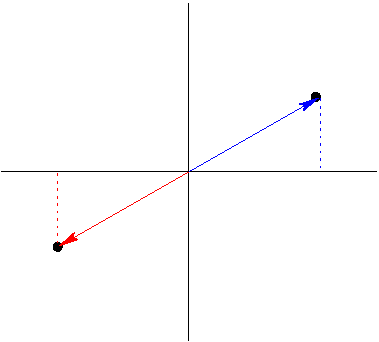
\includegraphics[scale=0.7]{figures/R2-rotate-pi.pdf}}
		\put(2.25,0.75){\scriptsize{$0$}}
		\put(2.05,1.6){\scriptsize{$y$}}
		\put(3.0,0.75){\scriptsize{$x$}}
		\put(2.85,1.22){\scriptsize{$(a,b)$}}
		\pause
		\put(1.0,0.5){\scriptsize{\alert{$(-a,-b)$}}}
		\end{picture}
		\pause
		
		We see that $ R_{\pi}\left[\begin{array}{c} a \\ b \end{array}\right]
		=
		\left[\begin{array}{c} -a \\ -b \end{array}\right]
		=
		\pause\left[\begin{array}{rr} -1 & 0 \\ 0 & -1 \end{array}\right]
		\left[\begin{array}{c} a \\ b \end{array}\right],$
		%so $R_{\pi}$ is a matrix transformation.
	\end{example}
}
%-------------- end slide -------------------------------%

%%-------------- start slide -------------------------------%
%\frame{\frametitle{Rotation}
%	\begin{problem}\em
%		The transformation $ R_{\frac{\pi}{2}}:\RR^2 \rightarrow \RR^2$
%		denotes a \alert{counterclockwise} rotation about the origin
%		through an angle of $\frac{\pi}{2}$ radians. Find the matrix of $R_{\frac{\pi}{2}}$.
%	\end{problem}
%	
%	\uncover<2->{
%		\begin{solution}\em
%			First, 
%			\[ R_{\frac{\pi}{2}}
%			\left[\begin{array}{c} a \\ b \end{array}\right]
%			=
%			\left[\begin{array}{r} -b \\ a \end{array}\right]
%			\]
%		}
%		\uncover<3->{Furthermore $R_{\frac{\pi}{2}}$ is a matrix
%			transformation, and the matrix it is induced by is 
%			\[ \left[\begin{array}{c} -b \\ a \end{array}\right] =
%			\left[\begin{array}{rr}
%			0 & -1 \\ 1 & 0 \end{array}\right]
%			\left[\begin{array}{c} a \\ b \end{array}\right]. \]}
%	\end{solution}
%}
%%-------------- end slide -------------------------------%


%-------------- start slide -------------------------------%
\frame{
	\begin{example}[Rotation through $\pi/2$]
		We denote by
		\[ R_{\pi/2}:\RR^2\to\RR^2\]
		counterclockwise rotation about the origin through an angle 
		of $\pi/2$.
		\pause
		\begin{picture}(4,1.75)
		\put(1.3,0.1){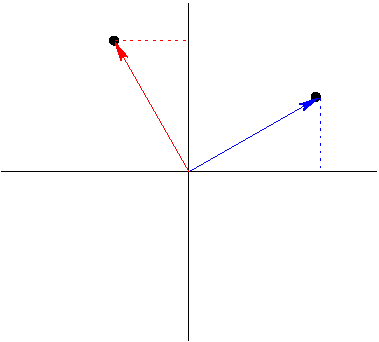
\includegraphics[scale=0.7]{figures/R2-rotate-halfpi.pdf}}
		\put(2.25,0.75){\scriptsize{$0$}}
		\put(2.05,1.6){\scriptsize{$y$}}
		\put(3.0,0.75){\scriptsize{$x$}}
		\put(2.85,1.22){\scriptsize{$(a,b)$}}
		\pause
		\put(1.4,1.5){\scriptsize{\alert{$(-b,a)$}}}
		\end{picture}
		\pause
		
		We see that $ R_{\pi/2}\left[\begin{array}{c} a \\ b \end{array}\right]
		=
		\left[\begin{array}{c} -b \\ a \end{array}\right]
		=
		\pause\left[\begin{array}{rr} 0 & -1 \\ 1 & 0 \end{array}\right]
		\left[\begin{array}{c} a \\ b \end{array}\right],$
		%so $R_{\pi/2}$ is a matrix transformation.
	\end{example}
}
%-------------- end slide -------------------------------%


\section{Reflections}

%--------------------start slide---------------------%
\frame{\frametitle{Reflection in $\RR^2$}
	\begin{example}
		In $\RR^2$, reflection in the $x$-axis, which transforms 
		$\left[\begin{array}{r} a \\ b \end{array}\right]$ to
		$\left[\begin{array}{r} a \\ -b \end{array}\right]$, 
		is a matrix transformation because
		\[ \left[\begin{array}{r} a \\ -b \end{array}\right] =
		\left[ \begin{array}{rr}
		1 & 0 \\ 0 & -1 \end{array}\right]
		\left[\begin{array}{r} a \\ b \end{array}\right].\]
	\end{example}
	\pause
	\begin{example}
		In $\RR^2$, reflection in the $y$-axis transforms 
		$\left[\begin{array}{r} a \\ b \end{array}\right]$ to
		$\left[\begin{array}{r} -a \\ b \end{array}\right]$.
		This is a matrix transformation because
		\[ \left[\begin{array}{r} -a \\ b \end{array}\right] =
		\left[ \begin{array}{rr}
		-1 & 0 \\ 0 & 1 \end{array}\right]
		\left[\begin{array}{r} a \\ b \end{array}\right].\]
	\end{example}
}
%-------------- end slide -------------------------------%

%-------------- start slide -------------------------------%
\frame{
	\begin{example}
		Reflection in the line $y=x$ 
		transforms
		$\left[\begin{array}{r} a \\ b \end{array}\right]$ to
		$\left[\begin{array}{r} b \\ a \end{array}\right]$.
		\bigskip
		
		\begin{picture}(4,1.5)
		\put(1.4,0){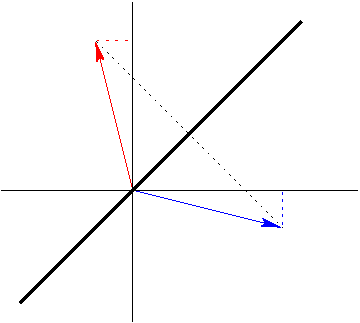
\includegraphics[scale=0.75]{figures/eigenvectors-2.pdf}}
		\put(2.85,0.45){\textcolor{blue}{{\scriptsize{$(a,b)$}}}}
		\put(1.55,1.4){\textcolor{red}{{\scriptsize{$(b,a)$}}}}
		\put(3.2,0.63){\scriptsize{$x$}}
		\put(2.1,1.5){\scriptsize{$y$}}
		\put(2.8,1.3){\scriptsize{$y=x$}}
		\end{picture}
		\pause
		
		This is a matrix transformation because
		\[ \left[\begin{array}{r} b \\ a \end{array}\right] =
		\left[ \begin{array}{rr}
		0 & 1 \\ 1 & 0 \end{array}\right]
		\left[\begin{array}{r} a \\ b \end{array}\right].\]
	\end{example}
}
%-------------- end slide -------------------------------%



%\section{Reflection in the line}
%%-------------- start slide -------------------------------%
%\frame{
%\begin{block}{Reflection in $y=mx$ preserves scalar multiplication}
%Let $Q_m:\RR^2\rightarrow \RR^2$ denote reflection in the
%line $y=mx$, and let $\vec{u}\in\RR^2$.
%\pause
%
%\begin{picture}(4,1.5)
%\uncover<2>{
%\put(0.3,0){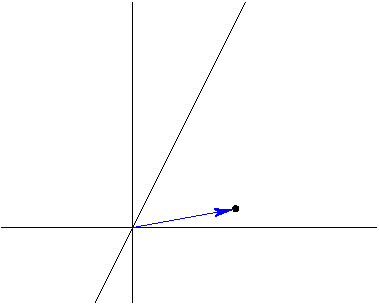
\includegraphics[scale=0.7]{figures/vectors-23a.pdf}}}
%\put(1.45,1.25){\scriptsize{$y=mx$}}
%\put(0.95,1.25){\scriptsize{$y$}}
%\put(1.95,0.25){\scriptsize{$x$}}
%\put(1.15,0.45){\scriptsize{\textcolor{blue}{$\vec{u}$}}}
%\uncover<3-5>{
%\put(0.3,0){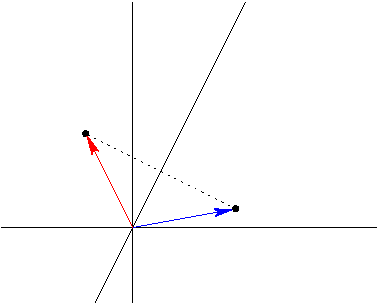
\includegraphics[scale=0.7]{figures/vectors-23b.pdf}}
%\put(0.4,0.55){\scriptsize{\textcolor{red}{$Q_m(\vec{u})$}}}
%}
%\uncover<4>{
%\put(2.5,0){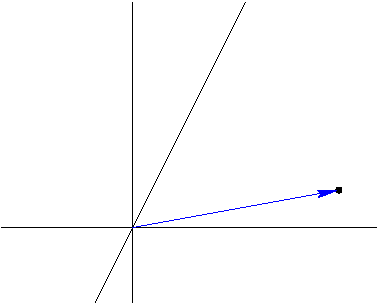
\includegraphics[scale=0.7]{figures/vectors-24a.pdf}}}
%\uncover<4->{
%\put(3.15,1.25){\scriptsize{$y$}}
%\put(4.15,0.25){\scriptsize{$x$}}
%\put(3.65,1.25){\scriptsize{$y=mx$}}
%\put(3.5,0.5){\scriptsize{\textcolor{blue}{$2\vec{u}$}}}}
%\uncover<5->{
%\put(2.5,0){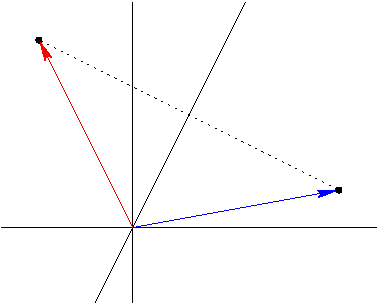
\includegraphics[scale=0.7]{figures/vectors-24.pdf}}
%\put(2.45,0.8){\scriptsize{\textcolor{red}{$Q_m(2\vec{u})$}}}}
%\uncover<6->{
%\put(0.3,0){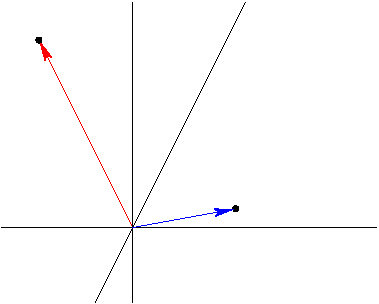
\includegraphics[scale=0.7]{figures/vectors-23.pdf}}
%\put(0.3,0.65){\scriptsize{\textcolor{red}{$2Q_m(\vec{u})$}}}
%}
%\end{picture}
%\bigskip
%
%\uncover<6->
%{The figure indicates that \alert{$Q_m(2\vec{u})=2Q_m(\vec{u})$.} }
%\uncover<7->
%{In general, for any scalar $k$, 
%\[ Q_m(kX)=kQ_m(X), \]}
%\uncover<8->
%{i.e., $Q_m$ preserves scalar multiplication.}
%\end{block}
%}
%%-------------- end slide -------------------------------%
%
%%-------------- start slide -------------------------------%
%\frame{
%\begin{block}{Reflection in $y=mx$ preserves vector addition}
%Let $\vec{u},\vec{v}\in\RR^2$.
%
%\begin{picture}(4,1.5)
%\uncover<2>{
%\put(0.3,0){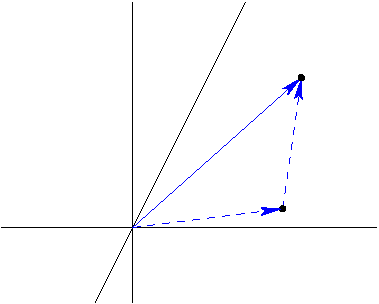
\includegraphics[scale=0.7]{figures/vectors-25a.pdf}}}
%\uncover<2->{
%\put(1.45,1.25){\scriptsize{$y=mx$}}
%\put(0.8,1.25){\scriptsize{$y$}}
%\put(1.95,0.25){\scriptsize{$x$}}
%\put(1.25,0.47){\scriptsize{\textcolor{blue}{$\vec{u}$}}}
%\put(1.7,0.7){\scriptsize{\textcolor{blue}{$\vec{v}$}}}
%\put(1.2,0.85){\scriptsize{\textcolor{blue}{$\vec{u}+\vec{v}$}}}}
%\uncover<3->{
%\put(0.3,0){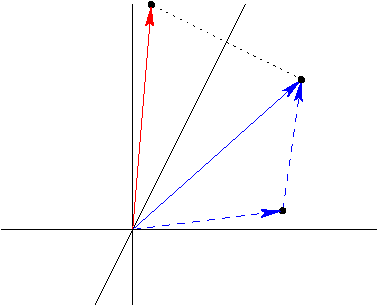
\includegraphics[scale=0.7]{figures/vectors-25.pdf}}
%\put(0.35,0.85){\scriptsize{\textcolor{red}{$Q_m(\vec{u}+\vec{v})$}}} }
%\uncover<4>{
%\put(2.5,0){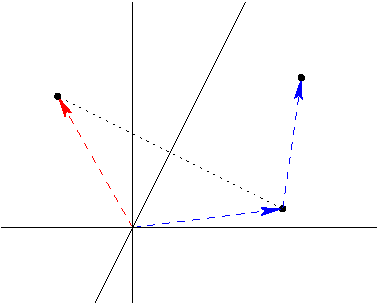
\includegraphics[scale=0.7]{figures/vectors-26a.pdf}}}
%\uncover<4->{
%\put(3.65,1.25){\scriptsize{$y=mx$}}
%\put(3.0,1.35){\scriptsize{$y$}}
%\put(4.15,0.25){\scriptsize{$x$}}
%\put(3.4,0.45){\scriptsize{\textcolor{blue}{$\vec{u}$}}}
%\put(3.9,0.7){\scriptsize{\textcolor{blue}{$\vec{v}$}}}
%\put(2.6,0.6){\scriptsize{\textcolor{red}{$Q_m(\vec{u})$}}}
%}
%\uncover<5>{
%\put(2.5,0){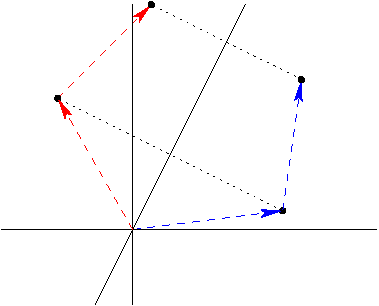
\includegraphics[scale=0.7]{figures/vectors-26b.pdf}}}
%\uncover<5->{
%\put(2.6,1.2){\scriptsize{\textcolor{red}{$Q_m(\vec{v})$}}}}
%\uncover<6->{
%\put(2.5,0){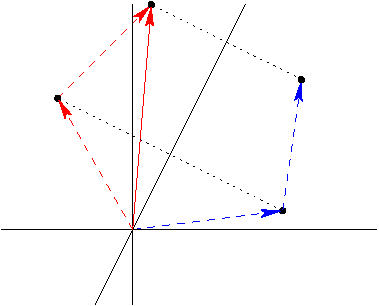
\includegraphics[scale=0.7]{figures/vectors-26c.pdf}}}
%%\uncover<7->{
%%\put(2.5,0){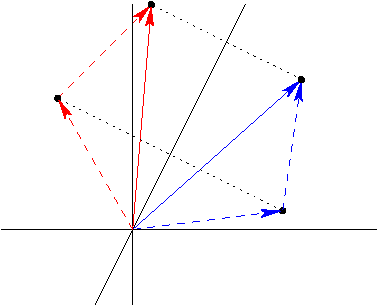
\includegraphics[scale=0.7]{figures/vectors-26.pdf}}}
%\end{picture}
%\bigskip
%
%\uncover<7->
%{The figure indicates that
%\alert{
%\[ Q_m(\vec{u}) + Q_m(\vec{v})=Q_m(\vec{u}+\vec{v}),\] } }
%\uncover<8->
%{i.e., $Q_m$ preserves vector addition.}
%\end{block}
%}
%%-------------- end slide -------------------------------%
%
%%-------------- start slide -------------------------------%
%\frame{
%\begin{block}{$Q_m$ is a linear transformation}
%Since $Q_m$ preserves addition and scalar multiplication,
%$Q_m$ is a linear transformation, and hence a matrix transformation.
%\bigskip
%\pause
%
%The matrix that induces $Q_m$ can be found by computing
%$Q_m(E_1)$ and $Q_m(E_2)$, where
%\[ 
%E_1=\left[\begin{array}{c} 1 \\ 0 \end{array}\right]
%~\mbox{ and }
%E_2=\left[\begin{array}{c} 0 \\ 1 \end{array}\right].
%\]
%\end{block}
%}
%%-------------- end slide -------------------------------%
%
%%-------------- start slide -------------------------------%
%\frame{
%\begin{block}{$Q_m(E_1)$}
%
%\begin{picture}(4,1.5)
%\uncover<1>{
%\put(1.3,0){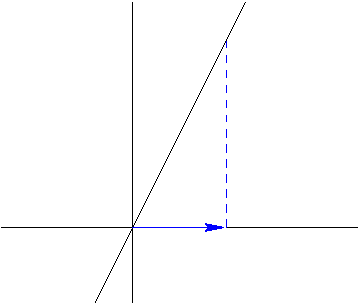
\includegraphics[scale=0.7]{figures/vectors-27a.pdf}}
%\put(2.0,0.38){\tiny{$\theta$}}}
%\uncover<1->{
%\put(2.45,1.25){\scriptsize{$y=mx$}}
%\put(1.8,1.25){\scriptsize{$y$}}
%\put(2.95,0.25){\scriptsize{$x$}} 
%\put(2.45,0.8){\scriptsize{\textcolor{blue}{$m$}}}
%\put(2.1,0.25){\scriptsize{\textcolor{blue}{$1$}}}
%}
%\uncover<2>{
%\put(1.3,0){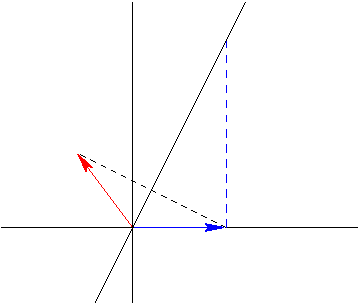
\includegraphics[scale=0.7]{figures/vectors-27b.pdf}}
%}
%\uncover<3->{
%\put(1.3,0){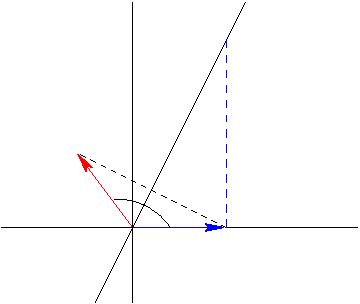
\includegraphics[scale=0.7]{figures/vectors-27c.pdf}}
%\put(2.1,0.38){\tiny{$2\theta$}}
%}
%\end{picture}
%
%\[ \cos\theta = \frac{1}{\sqrt{1+m^2}}
%~\mbox{ and }~ 
%\sin\theta = \frac{m}{\sqrt{1+m^2}} \]
%\[ \uncover<4->{
% Q_m(E_1) =\left[\begin{array}{c}
%\cos(2\theta) \\ \sin(2\theta) \end{array}\right]}
%\uncover<5->{
%=\left[\begin{array}{c}
%\cos^2\theta-\sin^2\theta \\ 2\sin\theta \cos\theta \end{array}\right]}
%\uncover<6->{
%=\frac{1}{1+m^2}\left[\begin{array}{c}
%1-m^2 \\ 2m \end{array}\right]}
%\]
%\end{block}
%}
%%-------------- end slide -------------------------------%
%
%%-------------- start slide -------------------------------%
%\frame{
%\begin{block}{$Q_m(E_2)$}
%\begin{picture}(4,1.5)
%\uncover<1>{
%\put(1.3,0){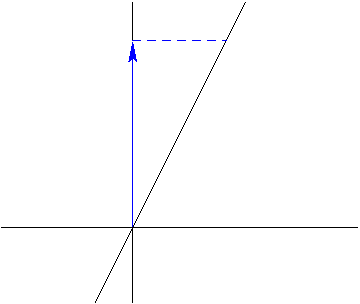
\includegraphics[scale=0.7]{figures/vectors-28a.pdf}} }
%\uncover<1->{
%\put(2.45,1.25){\scriptsize{$y=mx$}}
%\put(1.8,1.25){\scriptsize{$y$}}
%\put(2.95,0.25){\scriptsize{$x$}}
%\put(1.93,0.5){\tiny{$\theta$}}
%\put(1.75,0.8){\scriptsize{\textcolor{blue}{$1$}}}
%\put(2.1,1.35){\scriptsize{\textcolor{blue}{$\frac{1}{m}$}}}
%}
%\uncover<2>{
%\put(1.3,0){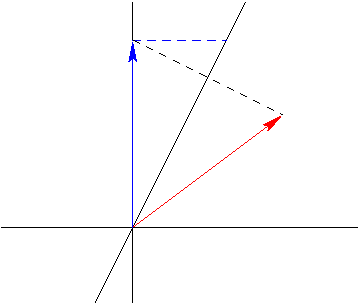
\includegraphics[scale=0.7]{figures/vectors-28b.pdf}}
%}
%\uncover<3->{
%\put(1.3,0){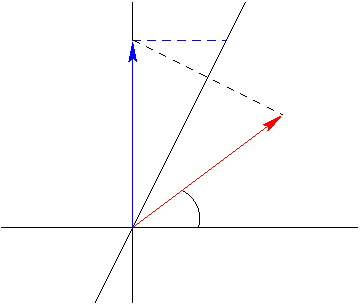
\includegraphics[scale=0.7]{figures/vectors-28c.pdf}}
%\put(2.26,0.43){\tiny{$\frac{\pi}{2}-2\theta$}} }
%\end{picture}
%
%\uncover<1->{
%\[ \cos\theta = \frac{m}{\sqrt{1+m^2}}
%~\mbox{ and }~
%\sin\theta = \frac{1}{\sqrt{1+m^2}} \]}
%\begin{eqnarray*}
%\uncover<4->{
% Q_m(E_2) & = & \left[\begin{array}{c}
%\cos(\frac{\pi}{2}-2\theta) \\ \sin(\frac{\pi}{2}-2\theta) \end{array}\right]}
%\uncover<5->{
%=\left[\begin{array}{c}
%\cos\frac{\pi}{2} \cos(2\theta)+\sin\frac{\pi}{2} \sin(2\theta) \\
%\sin\frac{\pi}{2} \cos(2\theta)-\cos\frac{\pi}{2} \sin(2\theta) \\
%\end{array}\right]} \\
%\uncover<6->{
%& = & \left[\begin{array}{c}
%\sin(2\theta) \\ \cos(2\theta) \end{array}\right]}
%\uncover<7->{
%=\left[\begin{array}{c}
%2\sin\theta \cos\theta \\ \cos^2\theta-\sin^2\theta  \end{array}\right]}
%\uncover<8->{
%=\frac{1}{1+m^2}\left[\begin{array}{c}
%2m \\ m^2-1 \end{array}\right]}
%\end{eqnarray*}
%\end{block}
%}
%%-------------- end slide -------------------------------%
%
%%-------------- start slide -------------------------------%
%\frame{
%\begin{block}{The Matrix for Reflection in $y=mx$}
%The transformation $Q_m:\RR^2\rightarrow\RR^2$,
%reflection in the line $y=mx$,
%is a linear transformation and is induced by the matrix
%\[ \frac{1}{1+m^2} 
%\left[\begin{array}{cc}
%1-m^2 & 2m \\ 2m & m^2-1
%\end{array}\right].\]
%\end{block}
%}
%%-------------- end slide -------------------------------%
%
%%-------------- start slide -------------------------------%
%\frame{\frametitle{Multiple Actions}
%\begin{problem}\em
%Find the rotation or reflection that equals reflection in the
%$x$-axis followed by rotation through an angle of $\frac{\pi}{2}$.
%\end{problem}
%
%\uncover<2->{
%\begin{solution}\em
%Let $Q_0$ denote the reflection in the $x$-axis, and $R_{\frac{\pi}{2}}$ denote the rotation through an angle of $\frac{\pi}{2}$. We want to find the matrix for the transformation
%$R_{\frac{\pi}{2}}\circ Q_0$.}
%
%\uncover<3->{
%$Q_0$ is induced by
%$A= \left[\begin{array}{rr}
%1 & 0 \\ 0 & -1
%\end{array}\right]$, and
%$R_{\frac{\pi}{2}}$ is induced by
%\[
%B=\left[\begin{array}{rr}
%\cos\frac{\pi}{2} & -\sin\frac{\pi}{2} \\
%\sin\frac{\pi}{2} & \cos\frac{\pi}{2}
%\end{array}\right]
%=
%\left[\begin{array}{rr}
%0 & -1 \\ 1 & 0
%\end{array}\right]
%\]}
%\end{solution}
%}
%%------------------end slide-------------------%
%
%%-------------------start slide--------------%
%\frame{
%\begin{solution}\em
%Hence $R_{\frac{\pi}{2}}\circ Q_0$ is induced by 
%\[ BA = 
%\left[\begin{array}{rr}
%0 & -1 \\ 1 & 0
%\end{array}\right]
%\left[\begin{array}{rr}
%1 & 0 \\ 0 & -1
%\end{array}\right]
%=
%\left[\begin{array}{rr}
%0 & 1 \\ 1 & 0
%\end{array}\right].\]
%
%\pause
%
%Notice that
%$BA= \left[\begin{array}{rr}
%0 & 1 \\ 1 & 0
%\end{array}\right]$
%is a \alert{reflection} matrix.
%
%\pause
%\begin{center}
%\alert{\Large How do we know this?}
%\end{center}
%
%\end{solution}
%}
%%-----------------end slide---------------%
%
%%-------------------start slide-------------%
%\frame{
%\begin{solution}[continued]\em
%
%Compare $BA$ to 
%\[ Q_m = \frac{1}{1+m^2}
%\left[\begin{array}{cc}
%1-m^2 & 2m \\ 2m & m^2-1
%\end{array}\right]
%\]
%
%
%\uncover<2->{
%Now, since $1-m^2=0$, we know that $m=1$ or $m=-1$.  
%But $\frac{2m}{1+m^2}=1>0$, so $m>0$, implying $m=1$.}
%\medskip
%
%\uncover<3->{
%Therefore, 
%\[ R_{\frac{\pi}{2}}\circ Q_0 = Q_1,\]
%reflection in the line $y=x$.}
%\end{solution}
%}
%%-------------- end slide -------------------------------%
%
%%-------------- start slide -------------------------------%
%\frame{\frametitle{Reflection followed by Reflection}
%\begin{problem}\em
%Find the rotation or reflection that equals reflection in the
%line $y=-x$ followed by reflection in the $y$-axis.
%\end{problem}
%
%\uncover<2->{
%\begin{solution}\em
%We must find the matrix for the transformation
%$Q_Y\circ Q_{-1}$.}
%\bigskip
%
%\uncover<3->{
%$Q_{-1}$ is induced by
%\[ A= \frac{1}{2}\left[\begin{array}{rr}
%0 & -2 \\ -2 & 0
%\end{array}\right]
%=
%\left[\begin{array}{rr}
%0 & -1 \\ -1 & 0
%\end{array}\right],
%\]
%and
%$Q_{Y}$ is induced by
%\[
%B=\left[\begin{array}{rr}
%-1 & 0 \\ 0 & 1
%\end{array}\right].
%\]}
%
%\uncover<4->{
%Therefore, $Q_Y\circ Q_{-1}$ is induced by $BA$.
%}
%\end{solution}
%}
%%-------------- end slide -------------------------------%
%
%%-------------- start slide -------------------------------%
%\frame{
%\begin{solution}[continued]\em
%\[ BA = \left[\begin{array}{rr}
%-1 & 0 \\ 0 & 1
%\end{array}\right]
%\left[\begin{array}{rr}
%0 & -1 \\ -1 & 0
%\end{array}\right]
%=
%\left[\begin{array}{rr}
%0 & 1 \\ -1 & 0
%\end{array}\right].\]
%\medskip
%
%\uncover<2->{
%\begin{center}
%\alert{\Large What transformation does $BA$ induce?}
%\end{center} }
%\medskip
%
%\uncover<3->{
%Rotation through an angle $\theta$ such that
%\[ \cos\theta = 0 \mbox{ and } \sin\theta = -1.\]
%}
%\medskip
%
%\uncover<4->{
%Therefore, $Q_Y\circ Q_{-1} = R_{-\frac{\pi}{2}} = 
%R_{\frac{3\pi}{2}}$.}
%\end{solution}
%}
%%-------------- end slide -------------------------------%
%
%%-------------- start slide -------------------------------%
%\frame{\frametitle{Summary}
%In general,
%\begin{itemize}
%\item The composite of two rotations is a \pause rotation
%\[
%R_\theta\circ R_\eta=R_{\theta+\eta}
%\]
%\pause
%\item <2-> The composite of two reflections is a \pause rotation.
%\[
%Q_m\circ Q_n = R_{\theta}
%\]
%where $\theta$ is $2\times$ the  angle between lines $y=mx$ and $y=nx$. 
%\bigskip
%\pause
%\item<3-> The composite of a reflection and a rotation is a \pause
%reflection.
%\[
%R_{\theta}\circ Q_n
%= 
%Q_m\circ Q_n\circ Q_n  
%=Q_m
%\]
%\end{itemize}
%}
%%-------------- end slide -------------------------------%

\end{document}
